\documentclass[Main.tex]{subfiles}
\begin{document}
	\gdef\muctieu{%
		\begin{enumerate}
			\item Nêu được khái niệm Khoa học tự nhiên.
			\item Trình bày được vai trò của Khoa học tự nhiên trong cuộc sống.
			\item Phân biệt được các lĩnh vực Khoa học tự nhiên dựa vào đối tượng nghiên cứu.
			\item Dựa vào các đặc điểm đặc trưng, phân biệt được vật sống và vật không sống.
			\item Nêu được các quy định an toàn khi học trong phòng thực hành.
			\item Phân biệt được các kí hiệu cảnh báo trong phòng thực hành.
			\item Đọc và phân biệt được các hình ảnh quy định an toàn phòng thực hành.
		\end{enumerate}
	}%
	\chapter{Mở đầu về khoa~học~tự~nhiên}
	\begin{Muctieu}
		\muctieu
	\end{Muctieu}
	\section{Giới thiệu về khoa học tự nhiên}
	\subsection{Lý Thuyết}
	\begin{kienthuccannho}
		\subsubsection{Khái niệm về khoa học tự nhiên}
			\begin{itemize}
				\item \textbf{\textit{Khoa học tự nhiên}} (KHTN) là ngành khoa học nghiên cứu các sự vật, hiện tượng, quy luật tự nhiên, những ảnh hưởng của tự nhiên đến cuộc sống con người và ngược lại.
				\item \textbf{Đối tượng nghiên cứu:} các sự vật, hiện tượng tự nhiên; các quá trình tự nhiên; các thuộc tính chung nhất về sự tồn tại, vận động của thế giới tự nhiên.
			\end{itemize}
		\subsubsection{Vật sống và vật không sống}
		\begin{center}
			\renewcommand{\arraystretch}{1.15}
			\begin{tabular}{|L{0.45\linewidth}|L{0.45\linewidth}|}
				\hline
				\textbf{\textit{Vật sống (vật hữu sinh):}}\
				Có các đặc trưng sống như trao đổi chất và năng lượng,
				sinh trưởng, phát triển, vận động, cảm ứng, sinh sản.
				&
				\textbf{\textit{Vật không sống (vật vô sinh):}}\
				Không có các đặc trưng trên.
				\\
				\hline
				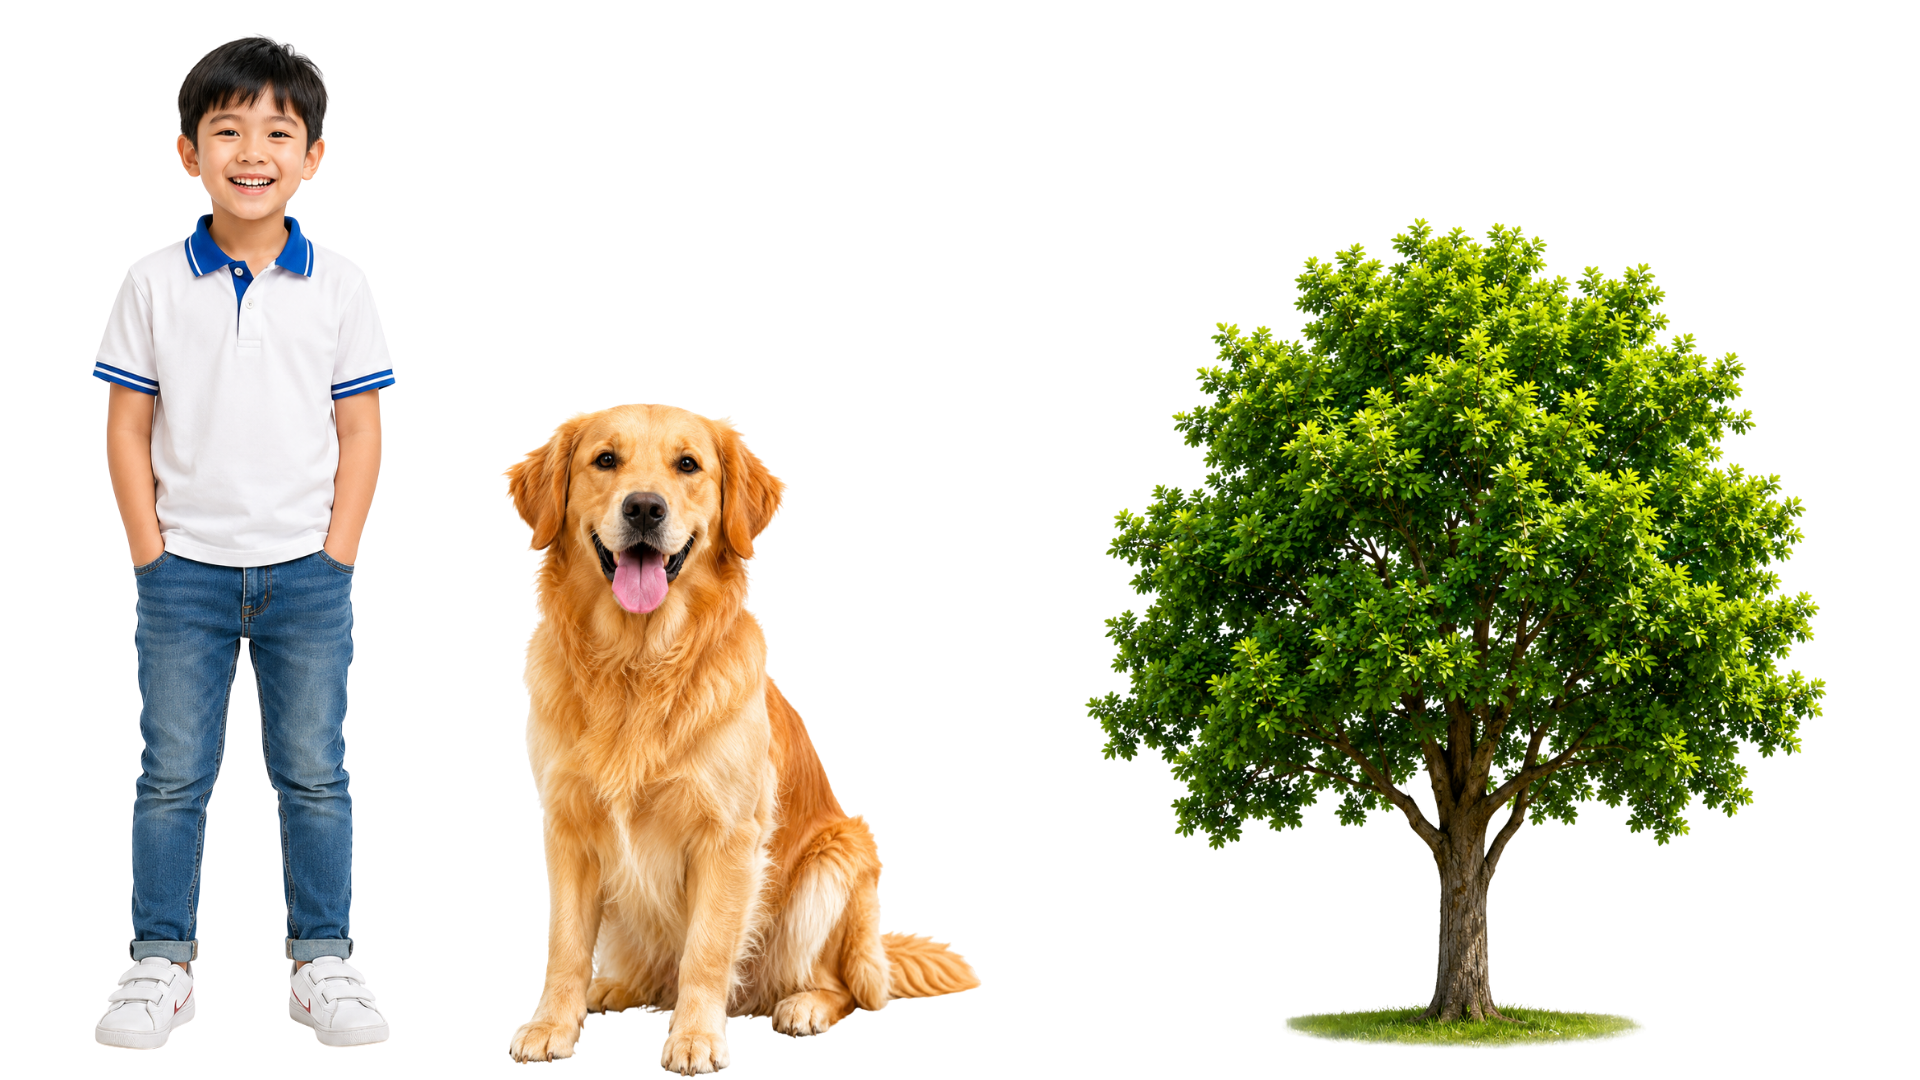
\includegraphics[
				width=0.95\linewidth
				]{Images/DE_CUONG_HOA_6_HKI/vat_song.png}
				&
				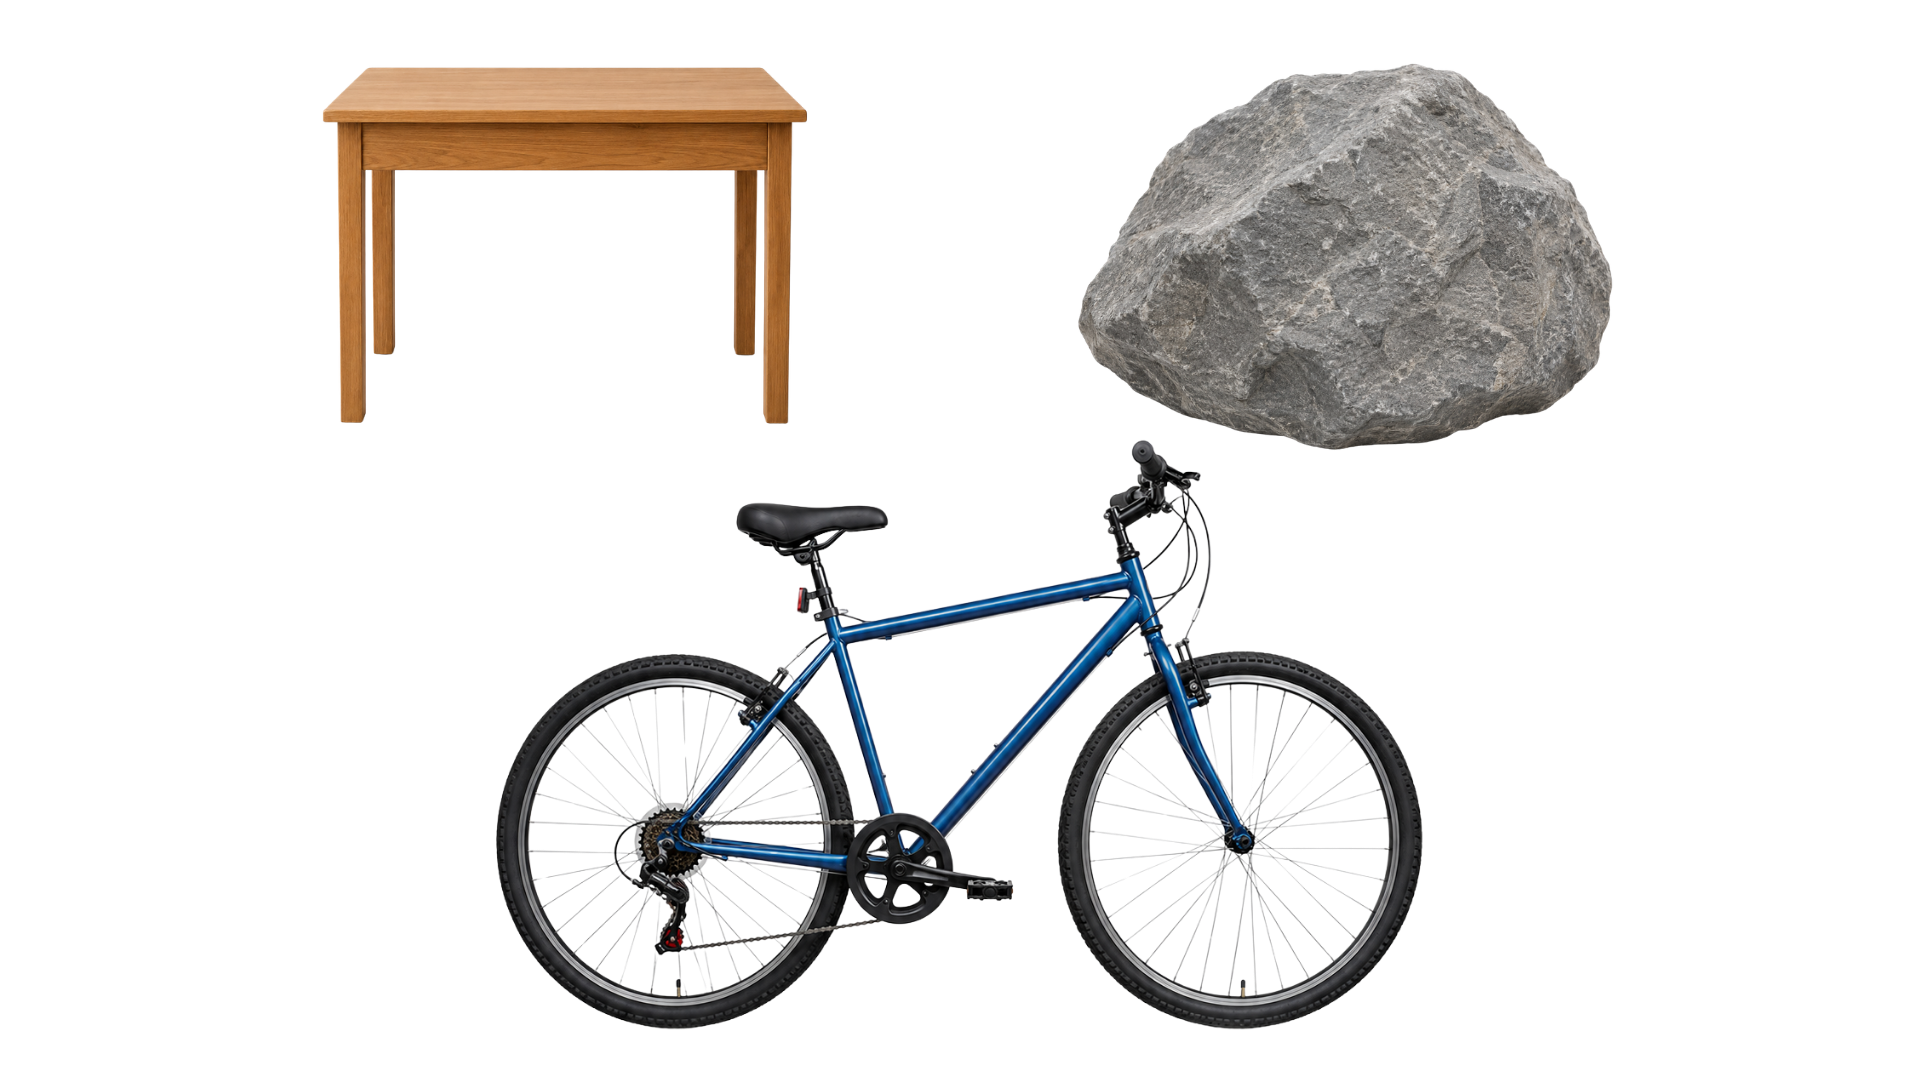
\includegraphics[
				width=0.95\linewidth
				]{Images/DE_CUONG_HOA_6_HKI/vat_khong_song.png}
				\\
				\hline
			\end{tabular}
		\end{center}
		\subsubsection{Các lĩnh vựa khác của khoa học tự nhiên}
		\begin{center}
			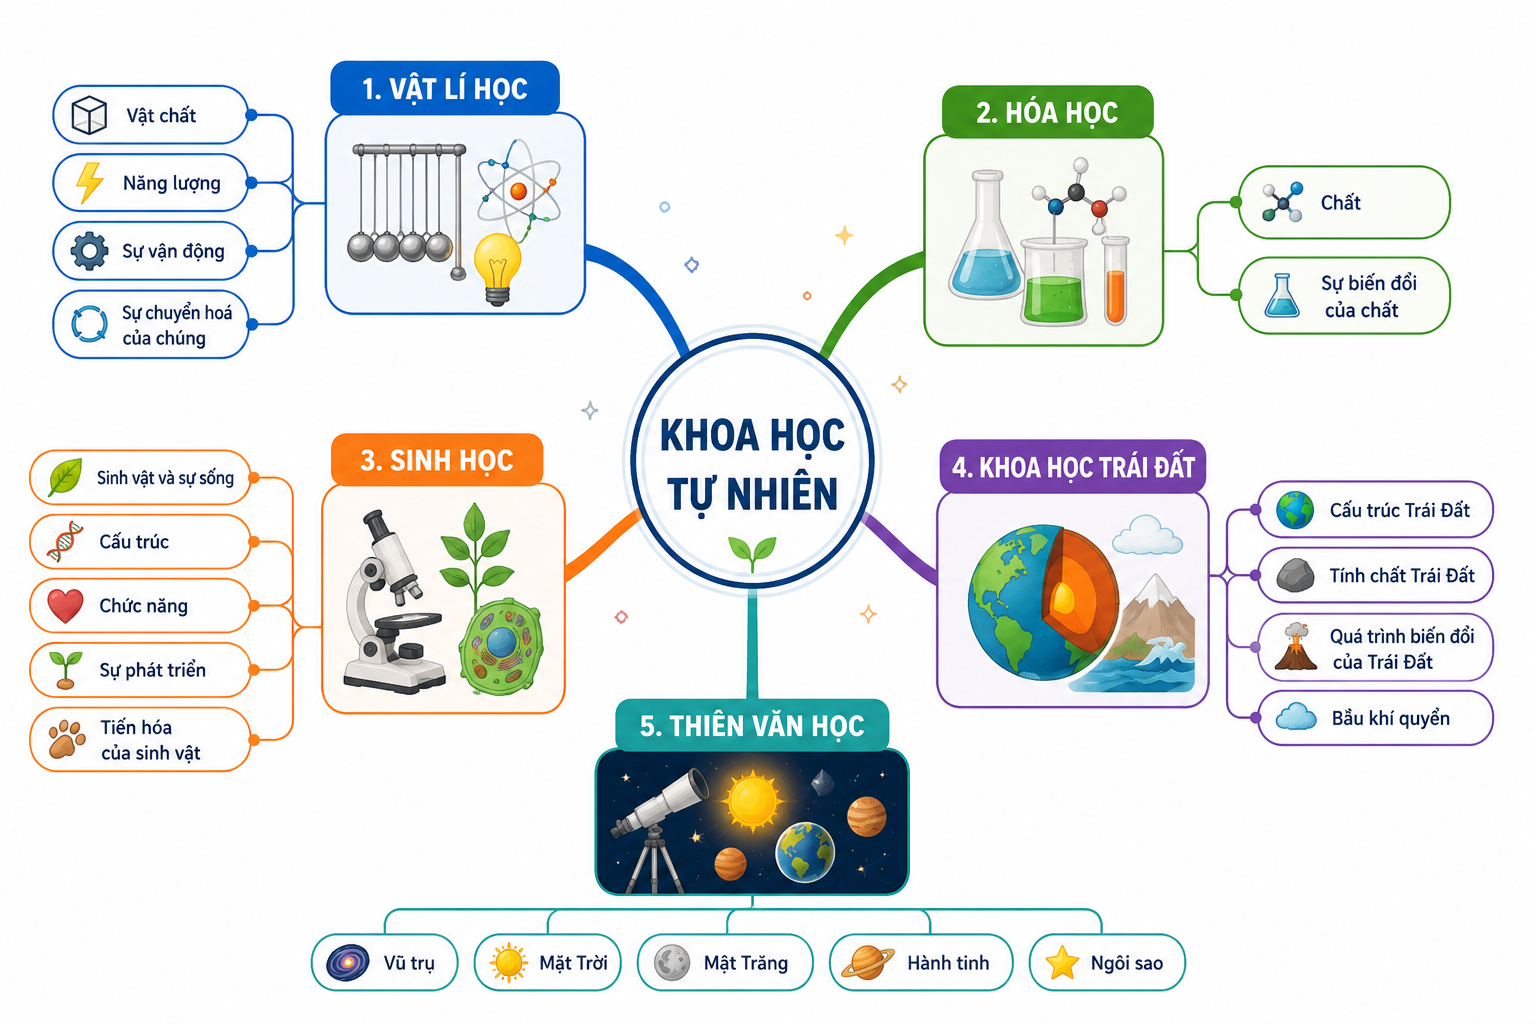
\includegraphics[
			width=0.98\linewidth
			]{Images/DE_CUONG_HOA_6_HKI/cac_linh_vuc_cua_khoa_hoc_tu_nhien.png}
		\end{center}
		\subsubsection{Khoa học tự nhiên với công nghệ và đời sống}
		\hspace{0.35cm}- Khoa học càng tiến bộ thì đời sống con người càng cải thiện. Tuy nhiên nếu sử dụng 
		không đúng phương pháp, đúng mục đích có thể gây hại tới môi trường tự nhiên và 
		con người. 
				\begin{center}
			\renewcommand{\arraystretch}{0.95}
			\begin{tabular}{C{0.45\linewidth}C{0.45\linewidth}}
				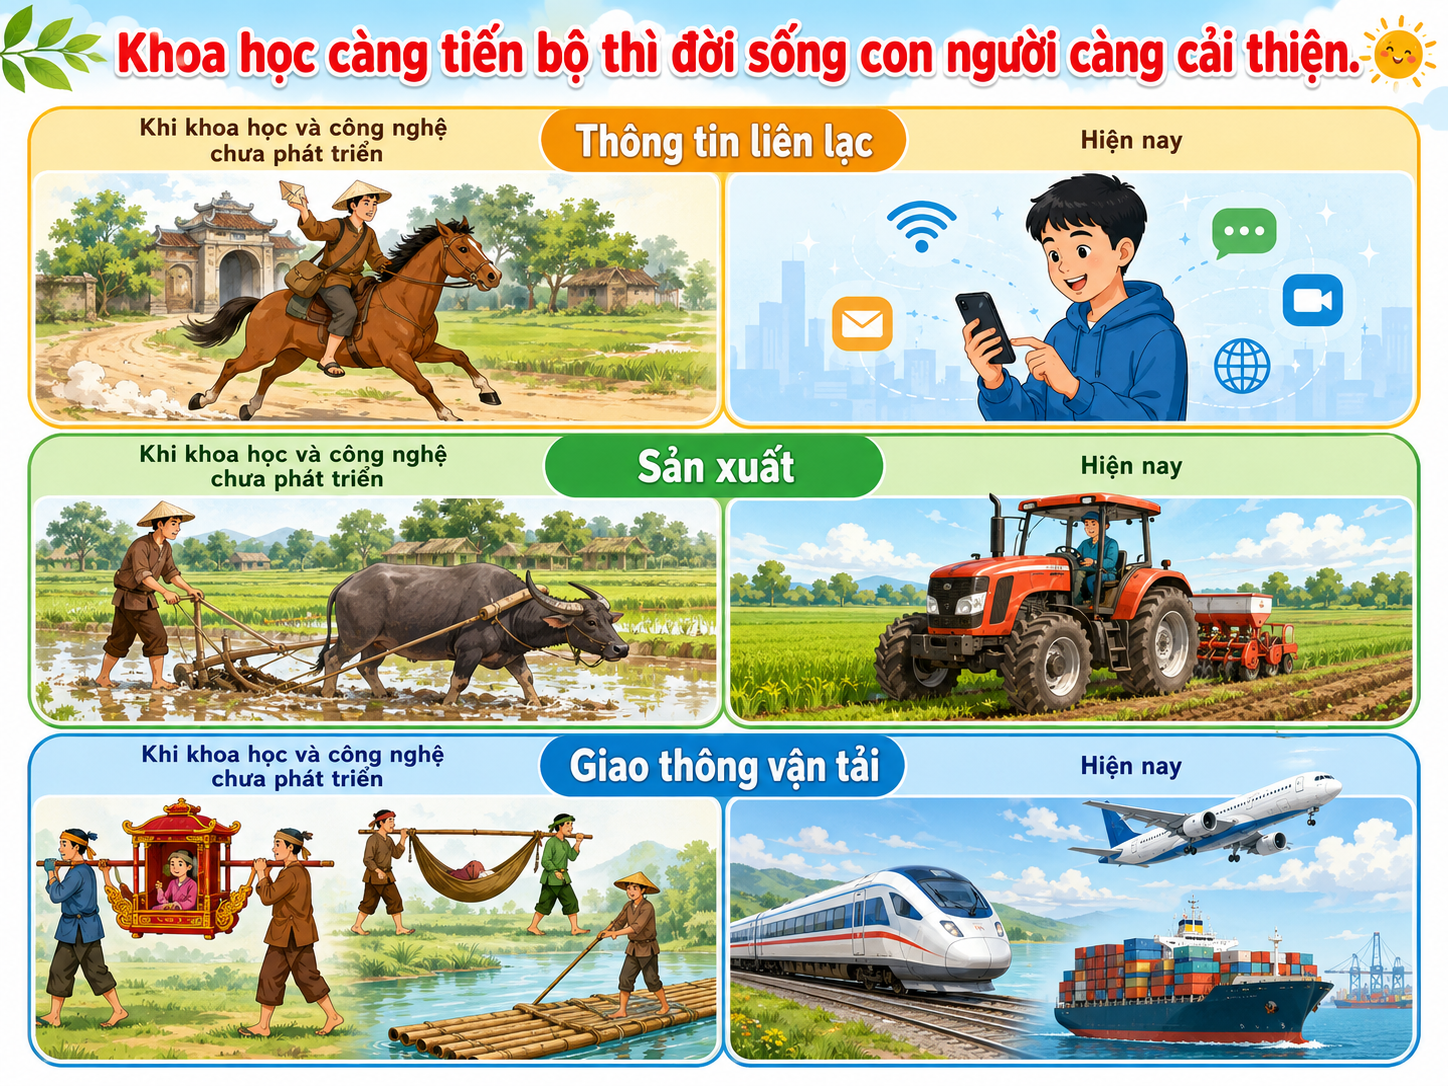
\includegraphics[
				width=0.95\linewidth
				]{Images/DE_CUONG_HOA_6_HKI/Vai_tro_cua_Khoa_hoc_cong_nghe.png}
				&
				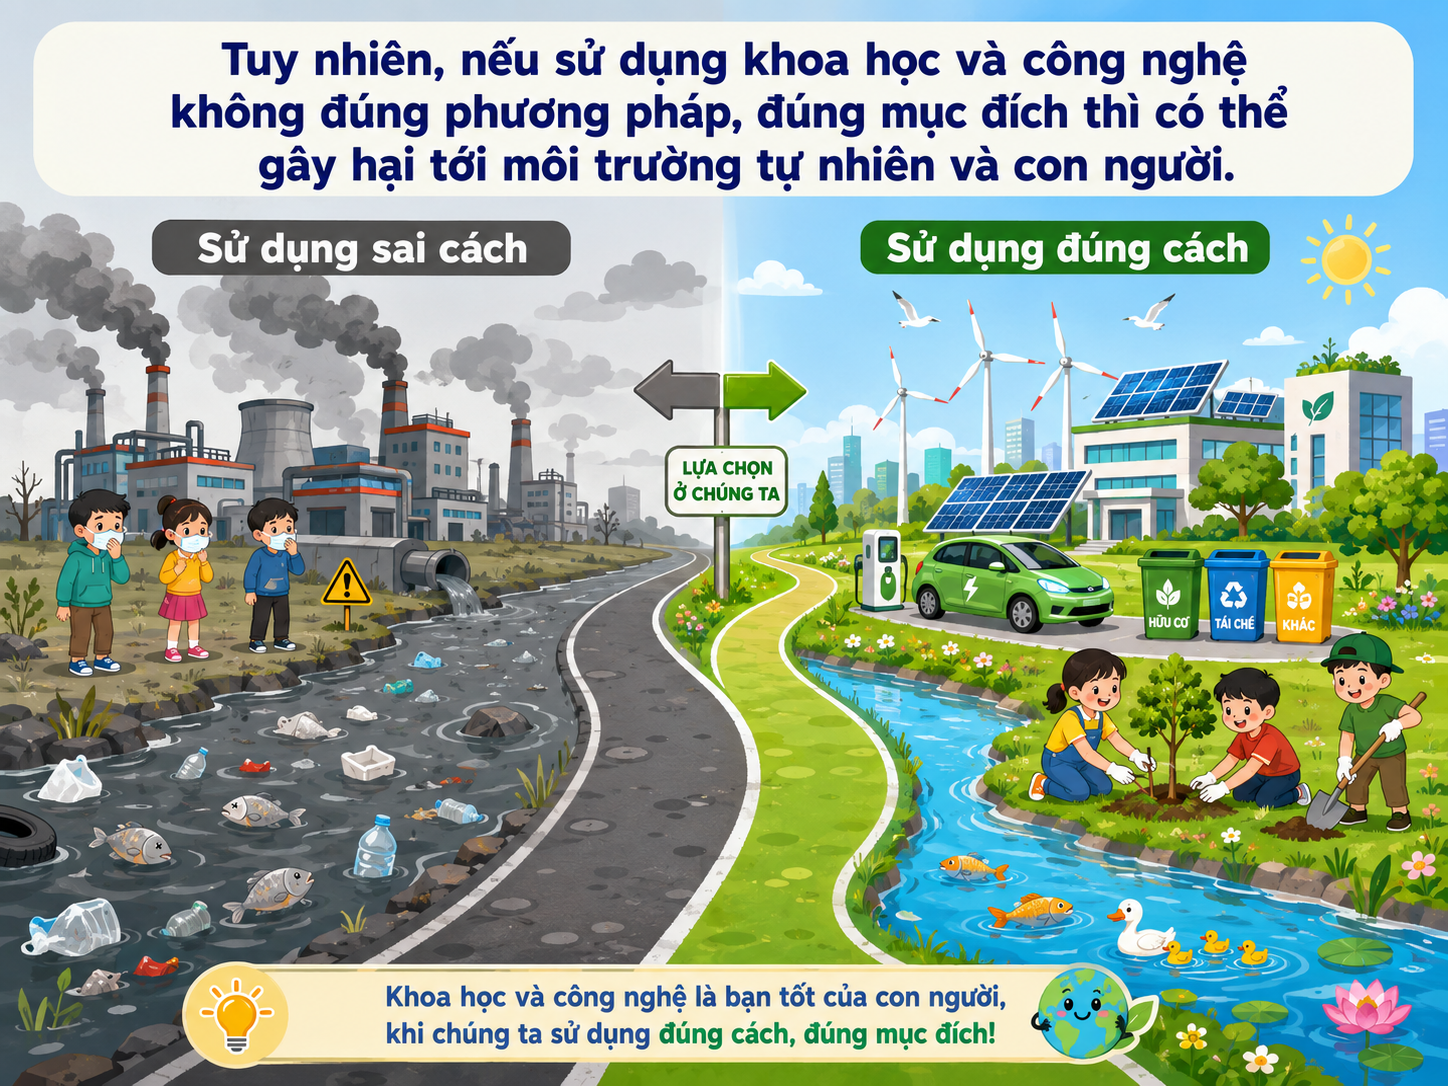
\includegraphics[
				width=0.95\linewidth
				]{Images/DE_CUONG_HOA_6_HKI/Vai_tro_cua_Khoa_hoc_cong_nghe_2.png}
				\\		
			\end{tabular}
		\end{center}
	\end{kienthuccannho}
	\subsection{Bài tập}
	
	%%%=================Phần bài tập tự luận===================%%%
	\phan{Bài tập tự luận}
	\textit{\large Thí sinh trả lời từ câu 1 đến câu 11}
	\Opensolutionfile{ansbth}[Ans/LGBT-C01_B01_MO_DAU_VE_KHTN]
	\Opensolutionfile{ansbt}[Ans/AnsBT-C01_B01_MO_DAU_VE_KHTN]
	%%%=============BT_1=============%%%
	\begin{bt}
		Khoa học tự nhiên là gì? Nêu một ví dụ về hoạt động nghiên cứu Khoa học tự nhiên mà em biết.
		\loigiai{
			Khoa học tự nhiên là ngành khoa học nghiên cứu các sự vật, hiện tượng, quy luật tự nhiên, những ảnh hưởng của tự nhiên đến cuộc sống con người và ngược lại.
			\\
			Ví dụ về hoạt động nghiên cứu Khoa học tự nhiên:
			\begin{itemize}
				\item Nghiên cứu sự nảy mầm của hạt đậu.
				\item Nghiên cứu sự bay hơi của nước dưới ánh nắng mặt trời.
			\end{itemize}
		}
	\end{bt}
	
	%%%=============BT_2=============%%%
	\begin{bt}
		Kể tên các lĩnh vực chủ yếu của Khoa học tự nhiên và đối tượng nghiên cứu của mỗi lĩnh vực.
		\loigiai{
			Các lĩnh vực chủ yếu của Khoa học tự nhiên và đối tượng nghiên cứu gồm:
			\begin{itemize}
				\item Vật lí học: nghiên cứu vật chất, năng lượng và sự vận động của chúng.
				\item Hoá học: nghiên cứu chất và sự biến đổi của chất.
				\item Sinh học: nghiên cứu sinh vật và sự sống.
				\item Khoa học Trái Đất: nghiên cứu Trái Đất và bầu khí quyển.
				\item Thiên văn học: nghiên cứu vũ trụ và các thiên thể.
			\end{itemize}
		}
	\end{bt}
	
	%%%=============BT_3=============%%%
	\begin{bt}
		Vì sao việc trồng cây xanh trong đô thị được xem là một ứng dụng của Khoa học tự nhiên?
		\loigiai{
			Việc trồng cây xanh trong đô thị được xem là một ứng dụng của Khoa học tự nhiên vì hoạt động này dựa trên hiểu biết của Sinh học.
			\\
			Cụ thể:
			\begin{itemize}
				\item Cây quang hợp, hấp thụ khí carbon dioxide.
				\item Cây thải khí oxygen.
				\item Cây góp phần cải thiện chất lượng không khí và điều hoà khí hậu.
			\end{itemize}
			Do đó, đây là việc ứng dụng kiến thức Khoa học tự nhiên vào bảo vệ môi trường và phục vụ đời sống con người.
		}
	\end{bt}
	
	%%%=============BT_4=============%%%
	\begin{bt}
		Em hãy phân biệt vật sống và vật không sống. Lấy $2$ ví dụ cho mỗi loại.
		\loigiai{
			Có thể phân biệt như sau:
			\begin{itemize}
				\item Vật sống có các đặc trưng: trao đổi chất và năng lượng, sinh trưởng, phát triển, vận động, cảm ứng, sinh sản.
				\item Vật không sống không có các đặc trưng nêu trên.
			\end{itemize}
			Ví dụ:
			\begin{itemize}
				\item Vật sống: cây lúa, con gà.
				\item Vật không sống: hòn đá, cái bàn.
			\end{itemize}
		}
	\end{bt}
	
	%%%=============BT_5=============%%%
	\begin{bt}
		Hiện tượng cây luôn vươn ngọn về phía có ánh sáng thể hiện đặc trưng nào của vật sống?
		\loigiai{
			Hiện tượng cây luôn vươn ngọn về phía có ánh sáng thể hiện tính cảm ứng.
			\\
			Đó là khả năng phản ứng của vật sống đối với kích thích từ môi trường, trong trường hợp này là ánh sáng.
		}
	\end{bt}
	
	%%%=============BT_6=============%%%
	\begin{bt}
		Em hãy lấy ví dụ $3$ hiện tượng hoặc vật thể thuộc lĩnh vực nghiên cứu của Hoá học và $3$ hiện tượng hoặc vật thể thuộc lĩnh vực nghiên cứu của Vật lí học.
		\loigiai{
			Ví dụ thuộc lĩnh vực nghiên cứu của Hoá học:
			\begin{itemize}
				\item Sắt bị gỉ.
				\item Đường tan trong nước.
				\item Nến cháy.
			\end{itemize}
			Ví dụ thuộc lĩnh vực nghiên cứu của Vật lí học:
			\begin{itemize}
				\item Quả bóng rơi xuống đất.
				\item Dòng điện thắp sáng bóng đèn.
				\item Nam châm hút đinh sắt.
			\end{itemize}
		}
	\end{bt}
	
	%%%=============BT_7=============%%%
	\begin{bt}
		Vì sao nói Khoa học tự nhiên có vai trò quan trọng trong đời sống? Lấy $2$ ví dụ minh hoạ.
		\loigiai{
			Khoa học tự nhiên có vai trò quan trọng trong đời sống vì cung cấp hiểu biết để ứng dụng vào chăm sóc sức khoẻ, bảo vệ môi trường, sản xuất, ...
			\\
			Ví dụ minh hoạ:
			\begin{itemize}
				\item Nghiên cứu vắc-xin phòng bệnh.
				\item Nghiên cứu giống cây trồng năng suất cao.
			\end{itemize}
		}
	\end{bt}
	
	%%%=============BT_8=============%%%
	\begin{bt}
		Vì sao nói việc phân biệt vật sống và vật không sống có ý nghĩa quan trọng trong học tập môn Khoa học tự nhiên?
		\loigiai{
			Việc phân biệt vật sống và vật không sống có ý nghĩa quan trọng vì đây là kiến thức nền tảng giúp học sinh nhận diện đúng đối tượng nghiên cứu của từng lĩnh vực, đặc biệt là Sinh học. Từ đó, học sinh vận dụng đúng phương pháp tìm hiểu phù hợp với từng loại đối tượng.
		}
	\end{bt}
	
	%%%=============BT_9=============%%%
	\begin{bt}
		Em hãy nêu $2$ ứng dụng của Khoa học tự nhiên trong đời sống hằng ngày mà em từng quan sát hoặc trải nghiệm.
		\loigiai{
			Một số ứng dụng của Khoa học tự nhiên trong đời sống hằng ngày:
			\begin{itemize}
				\item Sử dụng hệ thống lọc nước để loại bỏ tạp chất, vi khuẩn trong nước sinh hoạt.
				\item Trồng rau bằng phương pháp thuỷ canh có hệ thống cảm biến tự động.
			\end{itemize}
			Trong đó, ứng dụng thứ nhất gắn với Hoá học và Sinh học; ứng dụng thứ hai gắn với Sinh học và Vật lí học.
		}
	\end{bt}
	
	%%%=============BT_10=============%%%
	\begin{bt}
		Em hãy lấy một ví dụ cho thấy hiểu biết Khoa học tự nhiên giúp con người ứng phó tốt hơn với biến đổi khí hậu.
		\loigiai{
			Ví dụ: nghiên cứu về sự nóng lên toàn cầu và hiệu ứng nhà kính giúp con người đề ra các biện pháp giảm phát thải khí carbon dioxide, trồng thêm cây xanh, sử dụng năng lượng tái tạo như năng lượng mặt trời và năng lượng gió.
			\\
			Đây là ứng dụng phối hợp giữa Vật lí học, Hoá học và Khoa học Trái Đất.
		}
	\end{bt}
	
	%%%=============BT_11=============%%%
	\begin{bt}
		Khi xem chương trình dự báo thời tiết, em thấy có thông tin về nhiệt độ, độ ẩm, hướng gió được dự đoán dựa trên các số liệu quan trắc khí quyển. Hoạt động dự báo thời tiết này liên quan chủ yếu đến lĩnh vực nào của Khoa học tự nhiên? Giải thích.
		\loigiai{
			\begin{itemize}
				\item Hoạt động dự báo thời tiết liên quan chủ yếu đến lĩnh vực Khoa học Trái Đất.
				\item \textbf{Giải thích:} đối tượng nghiên cứu ở đây là bầu khí quyển cùng các hiện tượng thời tiết, khí hậu của Trái Đất.
			\end{itemize}
		}
	\end{bt}
	\Closesolutionfile{ansbt}
	\Closesolutionfile{ansbth}
	
	%%%=================Phần trắc nghiệm nhiều lựa chọn===================%%%
	\phan{Bài tập trắc nghiệm nhiều lựa chọn}
	\textit{\large Thí sinh trả lời từ câu 1 đến câu 25. Mỗi câu thí sinh chỉ chọn một phương án}
	\Opensolutionfile{ansex}[Ans/LGEX-C01_B01_MO_DAU_VE_KHTN]
	\Opensolutionfile{ans}[Ans/Ans-C01_B01_MO_DAU_VE_KHTN]
	%%%=============EX_1=============%%%
	\begin{ex}
		Khoa học tự nhiên là ngành khoa học nghiên cứu về
		\choice
		{các hiện tượng xã hội}
		{\True các sự vật, hiện tượng, quy luật tự nhiên}
		{các hoạt động kinh tế}
		{ngôn ngữ và văn hoá}
		\loigiai{Khoa học tự nhiên nghiên cứu các sự vật, hiện tượng và quy luật diễn ra trong tự nhiên.}
	\end{ex}
	
	%%%=============EX_2=============%%%
	\begin{ex}
		Lĩnh vực nào của Khoa học tự nhiên nghiên cứu về chất và sự biến đổi của chất?
		\choice
		{Vật lí học}
		{\True Hoá học}
		{Sinh học}
		{Thiên văn học}
		\loigiai{Hoá học nghiên cứu chất, tính chất của chất và sự biến đổi của chất.}
	\end{ex}
	
	%%%=============EX_3=============%%%
	\begin{ex}
		Lĩnh vực nào của Khoa học tự nhiên nghiên cứu về sinh vật và sự sống?
		\choice
		{Hoá học}
		{Vật lí học}
		{\True Sinh học}
		{Khoa học Trái Đất}
		\loigiai{Sinh học là lĩnh vực nghiên cứu sinh vật và các hoạt động sống.}
	\end{ex}
	
	%%%=============EX_4=============%%%
	\begin{ex}
		Lĩnh vực nào nghiên cứu về vật chất, năng lượng và sự vận động của chúng?
		\choice
		{\True Vật lí học}
		{Hoá học}
		{Sinh học}
		{Thiên văn học}
		\loigiai{Vật lí học nghiên cứu vật chất, năng lượng, lực và các quy luật vận động.}
	\end{ex}
	
	%%%=============EX_5=============%%%
	\begin{ex}
		Đối tượng nghiên cứu của Thiên văn học là
		\choice
		{Trái Đất và bầu khí quyển}
		{\True vũ trụ, các thiên thể}
		{chất và sự biến đổi của chất}
		{sinh vật và sự sống}
		\loigiai{Thiên văn học nghiên cứu vũ trụ và các thiên thể như Mặt Trời, Mặt Trăng, các hành tinh, sao.}
	\end{ex}
	
	%%%=============EX_6=============%%%
	\begin{ex}
		Đặc trưng nào sau đây KHÔNG phải là đặc trưng của vật sống?
		\choice
		{Trao đổi chất và năng lượng}
		{Sinh trưởng và phát triển}
		{Cảm ứng}
		{\True Có khối lượng lớn hơn 1 kg}
		\loigiai{Khối lượng lớn hay nhỏ không quyết định vật đó có sống hay không; còn trao đổi chất, sinh trưởng, cảm ứng là đặc trưng của vật sống.}
	\end{ex}
	
	%%%=============EX_7=============%%%
	\begin{ex}
		Vật thể nào sau đây là vật sống?
		\choice
		{\True Cây tre}
		{Cái ghế}
		{Ngọn núi}
		{Đám mây}
		\loigiai{Cây tre là sinh vật, có các đặc trưng sống như trao đổi chất, sinh trưởng và sinh sản.}
	\end{ex}
	
	%%%=============EX_8=============%%%
	\begin{ex}
		Việc sử dụng kính hiển vi để quan sát tế bào thuộc lĩnh vực nghiên cứu nào của Khoa học tự nhiên?
		\choice
		{Vật lí học}
		{Hoá học}
		{\True Sinh học}
		{Thiên văn học}
		\loigiai{Tế bào là đơn vị cấu tạo của cơ thể sống nên việc quan sát tế bào thuộc lĩnh vực Sinh học.}
	\end{ex}
	
	%%%=============EX_9=============%%%
	\begin{ex}
		Hoạt động nào sau đây thuộc lĩnh vực Hoá học?
		\choice
		{Quan sát sự sinh trưởng của cây đậu}
		{\True Nghiên cứu sự thay đổi màu sắc khi trộn hai dung dịch}
		{Quan sát chuyển động của các vì sao}
		{Đo tốc độ của một chiếc xe}
		\loigiai{Sự thay đổi màu sắc khi trộn hai dung dịch cho thấy có biến đổi của chất, thuộc lĩnh vực Hoá học.}
	\end{ex}
	
	%%%=============EX_10=============%%%
	\begin{ex}
		Vì sao việc phân loại vật sống và vật không sống chỉ dựa vào \lq\lq khả năng di chuyển\rq\rq\ là chưa chính xác?
		\choice
		{Vì mọi vật sống đều di chuyển được}
		{\True Vì có những vật sống không di chuyển được như cây xanh nhưng vẫn có các đặc trưng sống khác}
		{Vì di chuyển là đặc trưng duy nhất của vật sống}
		{Vì vật không sống luôn di chuyển được}
		\loigiai{Nhiều vật sống như cây xanh không di chuyển từ nơi này sang nơi khác nhưng vẫn trao đổi chất, sinh trưởng, cảm ứng và sinh sản.}
	\end{ex}
	
	%%%=============EX_11=============%%%
	\begin{ex}
		Việc dự báo thời tiết chủ yếu dựa trên nghiên cứu của lĩnh vực nào?
		\choice
		{Sinh học}
		{Hoá học}
		{\True Khoa học Trái Đất}
		{Thiên văn học}
		\loigiai{Dự báo thời tiết gắn với nghiên cứu khí quyển, thời tiết và khí hậu của Trái Đất nên thuộc Khoa học Trái Đất.}
	\end{ex}
	
	%%%=============EX_12=============%%%
	\begin{ex}
		Vì sao nói Khoa học tự nhiên góp phần thúc đẩy giáo dục STEM?
		\choice
		{Vì Khoa học tự nhiên không liên quan đến Toán học và Công nghệ}
		{\True Vì Khoa học tự nhiên cùng Toán học, Công nghệ, Tin học tạo nền tảng liên môn để giải quyết vấn đề thực tiễn}
		{Vì Khoa học tự nhiên chỉ dạy lí thuyết}
		{Vì giáo dục STEM không cần kiến thức khoa học}
		\loigiai{Giáo dục STEM cần kiến thức liên môn; Khoa học tự nhiên là một nền tảng quan trọng để giải quyết vấn đề thực tiễn.}
	\end{ex}
	
	%%%=============EX_13=============%%%
	\begin{ex}
		Hoạt động quan sát sự nảy mầm và phát triển của hạt đậu thuộc lĩnh vực nào?
		\choice
		{\True Sinh học}
		{Vật lí học}
		{Hoá học}
		{Thiên văn học}
		\loigiai{Sự nảy mầm và phát triển của hạt đậu là hoạt động sống của sinh vật nên thuộc Sinh học.}
	\end{ex}
	
	%%%=============EX_14=============%%%
	\begin{ex}
		Hoạt động nghiên cứu sự biến đổi của đá và sự hình thành núi lửa thuộc lĩnh vực nào?
		\choice
		{Hoá học}
		{Sinh học}
		{Vật lí học}
		{\True Khoa học Trái Đất}
		\loigiai{Đá, núi lửa và các quá trình diễn ra trong lòng đất là đối tượng nghiên cứu của Khoa học Trái Đất.}
	\end{ex}
	
	%%%=============EX_15=============%%%
	\begin{ex}
		Hoạt động đo tốc độ chuyển động của một chiếc xe đồ chơi chủ yếu liên quan đến lĩnh vực nào?
		\choice
		{\True Vật lí học}
		{Sinh học}
		{Thiên văn học}
		{Hoá học}
		\loigiai{Đo tốc độ là nghiên cứu chuyển động, thuộc phạm vi của Vật lí học.}
	\end{ex}
	
	%%%=============EX_16=============%%%
	\begin{ex}
		Cho các phát biểu:
		\begin{enumerate}
			\item[(a)] Robot là vật sống vì có thể \lq\lq di chuyển\rq\rq\ và \lq\lq phản ứng\rq\rq\ với môi trường.
			\item[(b)] Vật sống có khả năng sinh sản để duy trì nòi giống.
			\item[(c)] Núi lửa phun trào là một hiện tượng thuộc Sinh học.
			\item[(d)] Con người vừa là vật thể tự nhiên vừa là vật sống.
		\end{enumerate}
		Số phát biểu đúng là
		\choice
		{1}
		{\True 2}
		{3}
		{4}
		\loigiai{Phát biểu (b) đúng vì sinh sản là đặc trưng của vật sống. Phát biểu (d) đúng vì con người tồn tại trong tự nhiên và là sinh vật. Phát biểu (a) sai vì robot không có đầy đủ đặc trưng sống. Phát biểu (c) sai vì núi lửa thuộc Khoa học Trái Đất. Vậy có $2$ phát biểu đúng.}
	\end{ex}
	
	%%%=============EX_17=============%%%
	\begin{ex}
		Hiện tượng \lq\lq sắt để lâu ngoài không khí bị gỉ\rq\rq\ thuộc lĩnh vực nghiên cứu nào của Khoa học tự nhiên? Vì sao?
		\choice
		{Vật lí học, vì sắt bị thay đổi vị trí}
		{\True Hoá học, vì đây là sự biến đổi chất (sắt thành gỉ sắt)}
		{Sinh học, vì sắt là vật sống}
		{Thiên văn học, vì có liên quan đến không khí}
		\loigiai{Sắt bị gỉ là quá trình tạo ra chất mới nên là sự biến đổi hoá học, thuộc lĩnh vực Hoá học.}
	\end{ex}
	
	%%%=============EX_18=============%%%
	\begin{ex}
		Việc quan sát chuyển động của Mặt Trăng quanh Trái Đất để dự đoán hiện tượng nguyệt thực thuộc lĩnh vực nào của Khoa học tự nhiên?
		\choice
		{Sinh học}
		{Hoá học}
		{Khoa học Trái Đất}
		{\True Thiên văn học}
		\loigiai{Nguyệt thực liên quan đến chuyển động và vị trí của các thiên thể nên thuộc Thiên văn học.}
	\end{ex}
	
	%%%=============EX_19=============%%%
	\begin{ex}
		Vì sao một hiện tượng tự nhiên có thể liên quan đến nhiều lĩnh vực khác nhau của Khoa học tự nhiên?
		\choice
		{\True Vì ranh giới giữa các lĩnh vực không tách biệt tuyệt đối, một hiện tượng có thể được nhìn nhận dưới nhiều góc độ nghiên cứu}
		{Vì các lĩnh vực không có mối liên hệ với nhau}
		{Vì Khoa học tự nhiên chỉ có một lĩnh vực duy nhất}
		{Vì các nhà khoa học chưa thống nhất cách phân chia lĩnh vực}
		\loigiai{Nhiều hiện tượng tự nhiên có nhiều mặt khác nhau nên có thể được nghiên cứu bằng kiến thức của nhiều lĩnh vực.}
	\end{ex}
	
	%%%=============EX_20=============%%%
	\begin{ex}
		Bạn An nhận định: \lq\lq Cây nến đang cháy là một vật sống vì nó toả nhiệt và phát sáng.\rq\rq Nhận định này đúng hay sai?
		\choice
		{Đúng, vì toả nhiệt là đặc trưng của vật sống}
		{\True Sai, vì cháy là quá trình biến đổi hoá học, không phải là biểu hiện của trao đổi chất, sinh trưởng, sinh sản như ở vật sống}
		{Đúng, vì phát sáng chỉ có ở vật sống}
		{Sai, vì nến không tồn tại trong tự nhiên}
		\loigiai{Cây nến cháy chỉ là quá trình phản ứng hoá học. Nó không có các đặc trưng sống như sinh trưởng, sinh sản hay trao đổi chất theo nghĩa sinh học.}
	\end{ex}
	
	%%%=============EX_21=============%%%
	\begin{ex}
		Việc nghiên cứu cấu tạo, tính chất của các loại đá, khoáng vật trong lòng đất thuộc lĩnh vực nào của Khoa học tự nhiên?
		\choice
		{Sinh học}
		{Vật lí học}
		{\True Khoa học Trái Đất}
		{Thiên văn học}
		\loigiai{Đá và khoáng vật trong lòng đất là đối tượng nghiên cứu của Khoa học Trái Đất.}
	\end{ex}
	
	%%%=============EX_22=============%%%
	\begin{ex}
		Hoạt động dự đoán thời điểm xảy ra nhật thực thuộc lĩnh vực nào?
		\choice
		{Sinh học}
		{Vật lí học}
		{Hoá học}
		{\True Thiên văn học}
		\loigiai{Nhật thực là hiện tượng liên quan đến vị trí và chuyển động của Mặt Trời, Mặt Trăng và Trái Đất nên thuộc Thiên văn học.}
	\end{ex}
	
	%%%=============EX_23=============%%%
	\begin{ex}
		Hoạt động quan sát sự ăn mòn kim loại thuộc lĩnh vực nào?
		\choice
		{\True Hoá học}
		{Sinh học}
		{Vật lí học}
		{Khoa học Trái Đất}
		\loigiai{Ăn mòn kim loại là sự biến đổi chất của kim loại nên thuộc lĩnh vực Hoá học.}
	\end{ex}
	
	%%%=============EX_24=============%%%
	\begin{ex}
		Hoạt động trồng rau sạch bằng phương pháp thuỷ canh chủ yếu liên quan đến lĩnh vực nào?
		\choice
		{Vật lí học}
		{\True Sinh học}
		{Thiên văn học}
		{Hoá học}
		\loigiai{Trồng rau thuỷ canh chủ yếu gắn với sinh trưởng và phát triển của cây trồng nên thuộc Sinh học.}
	\end{ex}
	
	%%%=============EX_25=============%%%
	\begin{ex}
		Cho các phát biểu:
		\begin{enumerate}
			\item[(a)] Robot là vật sống vì có thể ``di chuyển'' và ``phản ứng'' với môi trường.
			\item[(b)] Vật sống có khả năng sinh sản để duy trì nòi giống.
			\item[(c)] Núi lửa phun trào là một hiện tượng thuộc Sinh học.
			\item[(d)] Con người vừa là vật thể tự nhiên vừa là vật sống.
		\end{enumerate}
		Số phát biểu đúng là
		\choice
		{1}
		{\True 2}
		{3}
		{4}
		\loigiai{Các phát biểu đúng là (b) và (d). Phát biểu (a) sai vì robot không có đầy đủ đặc trưng sống. Phát biểu (c) sai vì núi lửa là đối tượng của Khoa học Trái Đất. Vậy đáp án là $2$.}
	\end{ex}
	\Closesolutionfile{ans}
	\Closesolutionfile{ansex}
	%\bangdapan{Ans-C01_B01_MO_DAU_VE_KHTN}
	
	
	%%%=================Phần trắc nghiệm đúng sai===================%%%
	\phan{Bài tập trắc nghiệm đúng sai}
	\textit{\large Thí sinh trả lời từ câu 1 đến câu <tổng câu loại 2>. Trong mỗi ý a), b), c), d) ở mỗi câu thí sinh chọn đúng hoặc sai}
	\Opensolutionfile{ansex}[Ans/LGTF-C01_B01_MO_DAU_VE_KHTN]
	\Opensolutionfile{ansbook}[Ansbook/AnsTF-C01_B01_MO_DAU_VE_KHTN]
	\Opensolutionfile{ans}[Ans/Tempt-C01_B01_MO_DAU_VE_KHTN]
	\setcounter{ex}{0}
	%%%=============TF_1=============%%%
	\begin{ex}
		Xét về các lĩnh vực của Khoa học tự nhiên, đánh giá các phát biểu sau:
		\choiceTF
		{\True Hoá học nghiên cứu về chất và sự biến đổi của chất}
		{Vật lí học nghiên cứu về sinh vật và sự sống}
		{\True Thiên văn học nghiên cứu về vũ trụ và các thiên thể}
		{Khoa học Trái Đất chỉ nghiên cứu về các hành tinh khác trong hệ Mặt Trời}
		\loigiai{
			\begin{itemchoice}[T1,F2,T3,F4]
				\itemch Hoá học nghiên cứu chất, tính chất của chất và các biến đổi của chất nên phát biểu đúng.
				\itemch Sinh vật và sự sống là đối tượng nghiên cứu của Sinh học, không phải Vật lí học.
				\itemch Thiên văn học nghiên cứu vũ trụ và các thiên thể nên phát biểu đúng.
				\itemch Khoa học Trái Đất nghiên cứu Trái Đất, khí quyển, địa chất và các quá trình liên quan, không chỉ các hành tinh khác.
		\end{itemchoice}}
	\end{ex}
	
	%%%=============TF_2=============%%%
	\begin{ex}
		Xét về vật sống và vật không sống, đánh giá các phát biểu sau:
		\choiceTF
		{\True Trao đổi chất và năng lượng là một đặc trưng của vật sống}
		{Một chiếc ô tô tự lái có thể tự di chuyển nên được xem là vật sống}
		{\True Sinh trưởng và phát triển là đặc trưng chỉ có ở vật sống}
		{Mọi vật thể tự nhiên đều là vật sống}
		\loigiai{
			\begin{itemchoice}[T1,F2,T3,F4]
				\itemch Vật sống luôn có trao đổi chất và năng lượng với môi trường nên phát biểu đúng.
				\itemch Ô tô tự lái chỉ là máy móc, không có đầy đủ đặc trưng sống như sinh trưởng hay sinh sản nên phát biểu sai.
				\itemch Sinh trưởng và phát triển là đặc trưng cơ bản của vật sống nên phát biểu đúng.
				\itemch Nhiều vật thể tự nhiên như hòn đá, nước, không khí không phải vật sống nên phát biểu sai.
		\end{itemchoice}}
	\end{ex}
	
	%%%=============TF_3=============%%%
	\begin{ex}
		Xét về đặc trưng của vật sống, đánh giá các phát biểu sau:
		\choiceTF
		{\True Vật sống có khả năng trao đổi chất và năng lượng với môi trường}
		{Vật sống không có khả năng sinh sản}
		{\True Sinh trưởng và phát triển là một trong các đặc trưng của vật sống}
		{Mọi vật thể tự nhiên đều được xem là vật sống}
		\loigiai{
			\begin{itemchoice}[T1,F2,T3,F4]
				\itemch Trao đổi chất và năng lượng là đặc trưng quan trọng của vật sống nên phát biểu đúng.
				\itemch Vật sống có khả năng sinh sản để duy trì nòi giống nên phát biểu sai.
				\itemch Sinh trưởng và phát triển là đặc trưng của vật sống nên phát biểu đúng.
				\itemch Vật thể tự nhiên không phải lúc nào cũng là vật sống; ví dụ hòn đá không sống.
		\end{itemchoice}}
	\end{ex}
	
	%%%=============TF_4=============%%%
	\begin{ex}
		Xét về lĩnh vực Vật lí học và Thiên văn học, đánh giá các phát biểu sau:
		\choiceTF
		{\True Vật lí học nghiên cứu về vật chất, lực và năng lượng}
		{\True Thiên văn học nghiên cứu về vũ trụ và các thiên thể}
		{Vật lí học và Thiên văn học là một lĩnh vực duy nhất, không phân biệt}
		{Nghiên cứu về Mặt Trời thuộc lĩnh vực Vật lí học, không liên quan đến Thiên văn học}
		\loigiai{
			\begin{itemchoice}[T1,T2,F3,F4]
				\itemch Vật lí học nghiên cứu vật chất, chuyển động, lực và năng lượng nên phát biểu đúng.
				\itemch Thiên văn học nghiên cứu các thiên thể và vũ trụ nên phát biểu đúng.
				\itemch Hai lĩnh vực có liên hệ nhưng vẫn là hai lĩnh vực khác nhau nên phát biểu sai.
				\itemch Mặt Trời là thiên thể nên nghiên cứu về Mặt Trời có liên quan rõ ràng đến Thiên văn học; phát biểu sai.
		\end{itemchoice}}
	\end{ex}
	
	%%%=============TF_5=============%%%
	\begin{ex}
		Xét về vai trò của Khoa học tự nhiên, đánh giá các phát biểu sau:
		\choiceTF
		{\True Khoa học tự nhiên giúp nâng cao hiểu biết của con người về thế giới tự nhiên}
		{Khoa học tự nhiên không có ứng dụng gì trong sản xuất nông nghiệp, công nghiệp}
		{\True Khoa học tự nhiên là nền tảng cho giáo dục STEM}
		{Khoa học tự nhiên chỉ có giá trị lí thuyết, không giúp ứng phó với biến đổi khí hậu}
		\loigiai{
			\begin{itemchoice}[T1,F2,T3,F4]
				\itemch Khoa học tự nhiên giúp con người hiểu thế giới tự nhiên nên phát biểu đúng.
				\itemch Khoa học tự nhiên có nhiều ứng dụng trong nông nghiệp, công nghiệp nên phát biểu sai.
				\itemch STEM cần nền tảng từ khoa học, công nghệ, kĩ thuật và toán học nên phát biểu đúng.
				\itemch Kiến thức Khoa học tự nhiên giúp dự báo, giảm thiểu và ứng phó với biến đổi khí hậu nên phát biểu sai.
		\end{itemchoice}}
	\end{ex}
	
	%%%=============TF_6=============%%%
	\begin{ex}
		Một trạm khí tượng theo dõi nhiệt độ, độ ẩm, tốc độ gió; trong khi một trại nghiên cứu nông nghiệp theo dõi sự phát triển của một giống lúa mới. Đánh giá các phát biểu sau:
		\choiceTF
		{\True Hoạt động của trạm khí tượng thuộc lĩnh vực Khoa học Trái Đất}
		{\True Hoạt động theo dõi giống lúa mới thuộc lĩnh vực Sinh học}
		{Cả hai hoạt động trên đều không liên quan đến Khoa học tự nhiên}
		{Hai hoạt động trên chỉ mang tính giải trí, không có ứng dụng thực tế}
		\loigiai{
			\begin{itemchoice}[T1,T2,F3,F4]
				\itemch Trạm khí tượng nghiên cứu thời tiết, khí quyển nên thuộc Khoa học Trái Đất.
				\itemch Theo dõi sự phát triển của giống lúa là nghiên cứu sinh vật nên thuộc Sinh học.
				\itemch Cả hai hoạt động đều thuộc Khoa học tự nhiên nên phát biểu sai.
				\itemch Hai hoạt động đều có ứng dụng thực tế trong dự báo thời tiết và sản xuất nông nghiệp nên phát biểu sai.
		\end{itemchoice}}
	\end{ex}
	
	%%%=============TF_7=============%%%
	\begin{ex}
		Một bạn học sinh quan sát thấy: lá cây trầu bà trồng trong nhà luôn vươn về phía cửa sổ có ánh sáng; trong khi một hòn đá cảnh đặt cạnh đó không có sự thay đổi nào. Đánh giá các phát biểu sau:
		\choiceTF
		{\True Hiện tượng lá cây vươn về phía ánh sáng thể hiện tính cảm ứng của vật sống}
		{\True Hòn đá không phản ứng vì đó là vật không sống}
		{Cả cây và hòn đá đều là vật sống vì cùng được đặt trong nhà}
		{Tính cảm ứng không phải là đặc trưng riêng của vật sống}
		\loigiai{
			\begin{itemchoice}[T1,T2,F3,F4]
				\itemch Cây phản ứng với ánh sáng nên thể hiện tính cảm ứng, đây là đặc trưng của vật sống.
				\itemch Hòn đá là vật không sống nên không có phản ứng sinh học như cây.
				\itemch Việc cùng đặt trong nhà không làm hòn đá trở thành vật sống nên phát biểu sai.
				\itemch Tính cảm ứng là một đặc trưng của vật sống nên phát biểu sai.
		\end{itemchoice}}
	\end{ex}
	
	%%%=============TF_8=============%%%
	\begin{ex}
		Một trạm quan trắc theo dõi độ rung chấn trong lòng đất để cảnh báo sớm động đất. Đánh giá các phát biểu sau:
		\choiceTF
		{\True Hoạt động này thuộc lĩnh vực Khoa học Trái Đất}
		{Hoạt động này không có ứng dụng thực tiễn}
		{\True Việc cảnh báo sớm giúp giảm thiểu thiệt hại về người và tài sản}
		{Chỉ có lĩnh vực Vật lí học mới liên quan đến hiện tượng động đất}
		\loigiai{
			\begin{itemchoice}[T1,F2,T3,F4]
				\itemch Động đất là hiện tượng xảy ra trong lòng đất nên thuộc Khoa học Trái Đất.
				\itemch Cảnh báo động đất có giá trị thực tiễn rất lớn nên phát biểu sai.
				\itemch Cảnh báo sớm giúp con người chủ động phòng tránh, giảm thiệt hại nên phát biểu đúng.
				\itemch Động đất không chỉ liên quan đến Vật lí học mà còn thuộc Khoa học Trái Đất nên phát biểu sai.
		\end{itemchoice}}
	\end{ex}
	
	%%%=============TF_9=============%%%
	\begin{ex}
		Xét tình huống: một nhóm học sinh trồng hai chậu cây giống nhau, một chậu tưới nước đều đặn, một chậu không tưới nước, sau đó so sánh sự phát triển. Đánh giá các phát biểu sau:
		\choiceTF
		{\True Đây là một ví dụ về phương pháp nghiên cứu khoa học bằng cách so sánh, đối chứng}
		{Kết quả thí nghiệm không liên quan đến Khoa học tự nhiên}
		{\True Hoạt động này thuộc lĩnh vực Sinh học vì đối tượng nghiên cứu là cây (sinh vật)}
		{Thí nghiệm này không cần có nhóm đối chứng vẫn cho kết quả đáng tin cậy}
		\loigiai{
			\begin{itemchoice}[T1,F2,T3,F4]
				\itemch Hai chậu cây được dùng để so sánh điều kiện có tưới và không tưới nên đây là thí nghiệm đối chứng.
				\itemch Thí nghiệm nghiên cứu sự phát triển của cây nên rõ ràng liên quan đến Khoa học tự nhiên.
				\itemch Cây là sinh vật nên hoạt động này thuộc lĩnh vực Sinh học.
				\itemch Nhóm đối chứng giúp so sánh và tăng độ tin cậy cho kết quả, vì vậy phát biểu sai.
		\end{itemchoice}}
	\end{ex}
	
	%%%=============TF_10=============%%%
	\begin{ex}
		Một nhóm học sinh thực hiện dự án ``Vườn rau thuỷ canh có cảm biến độ ẩm tự động''. Đánh giá các phát biểu sau:
		\choiceTF
		{\True Việc theo dõi sự sinh trưởng của rau thuộc lĩnh vực Sinh học}
		{\True Việc thiết kế cảm biến, mạch điện đo độ ẩm thuộc lĩnh vực Vật lí học}
		{Dự án này không thể hiện vai trò của Khoa học tự nhiên trong đời sống}
		{Dự án chỉ sử dụng kiến thức của một lĩnh vực Khoa học tự nhiên duy nhất}
		\loigiai{
			\begin{itemchoice}[T1,T2,F3,F4]
				\itemch Sự sinh trưởng của rau là quá trình sống nên thuộc Sinh học.
				\itemch Cảm biến và mạch điện liên quan đến đo đạc, điện học nên thuộc Vật lí học.
				\itemch Dự án cho thấy ứng dụng của Khoa học tự nhiên trong trồng trọt nên phát biểu sai.
				\itemch Dự án dùng kiến thức của nhiều lĩnh vực như Sinh học và Vật lí học nên phát biểu sai.
		\end{itemchoice}}
	\end{ex}
	
	%%%=============TF_11=============%%%
	\begin{ex}
		Một nhóm học sinh thực hiện dự án tìm hiểu vì sao chim én thường bay thấp trước khi trời mưa. Đánh giá các phát biểu sau:
		\choiceTF
		{\True Đây là một hiện tượng tự nhiên có thể được nghiên cứu dưới góc độ Sinh học (tập tính động vật) và Khoa học Trái Đất (độ ẩm, áp suất khí quyển trước mưa)}
		{Hiện tượng này chỉ có thể giải thích bằng một lĩnh vực Khoa học tự nhiên duy nhất}
		{Việc quan sát tập tính động vật để dự đoán thời tiết hoàn toàn không liên quan đến Khoa học tự nhiên}
		{\True Kết quả nghiên cứu của dự án có thể góp phần vào việc dự báo thời tiết dựa trên quan sát tự nhiên}
		\loigiai{
			\begin{itemchoice}[T1,F2,F3,T4]
				\itemch Hiện tượng này liên quan cả tập tính sinh vật lẫn điều kiện khí quyển nên phát biểu đúng.
				\itemch Một hiện tượng có thể được nghiên cứu dưới nhiều góc độ nên phát biểu sai.
				\itemch Quan sát tập tính động vật và thời tiết đều thuộc Khoa học tự nhiên nên phát biểu sai.
				\itemch Kết quả nghiên cứu có thể hỗ trợ dự báo thời tiết từ dấu hiệu tự nhiên nên phát biểu đúng.
		\end{itemchoice}}
	\end{ex}
	
	%%%=============TF_12=============%%%
	\begin{ex}
		Một bác sĩ sử dụng nhiệt kế điện tử đo thân nhiệt, đồng thời quan sát các biểu hiện của cơ thể để chẩn đoán bệnh cho bệnh nhân. Đánh giá các phát biểu sau:
		\choiceTF
		{\True Việc đo thân nhiệt bằng nhiệt kế liên quan đến kiến thức Vật lí học}
		{\True Việc quan sát các biểu hiện của cơ thể người liên quan đến kiến thức Sinh học}
		{Hoạt động khám chữa bệnh hoàn toàn không liên quan đến Khoa học tự nhiên}
		{\True Đây là một minh chứng cho vai trò của Khoa học tự nhiên trong chăm sóc sức khoẻ con người}
		\loigiai{
			\begin{itemchoice}[T1,T2,F3,T4]
				\itemch Nhiệt kế đo nhiệt độ là ứng dụng của kiến thức Vật lí học nên phát biểu đúng.
				\itemch Quan sát cơ thể người gắn với hoạt động sống nên liên quan đến Sinh học.
				\itemch Khám chữa bệnh sử dụng nhiều kiến thức Khoa học tự nhiên nên phát biểu sai.
				\itemch Đây là ví dụ rõ về ứng dụng Khoa học tự nhiên trong chăm sóc sức khoẻ nên phát biểu đúng.
		\end{itemchoice}}
	\end{ex}
	
	%%%=============TF_13=============%%%
	\begin{ex}
		Cho tình huống: Một khu vườn trường có trồng nhiều loại cây, có một tấm biển ghi kí hiệu cảnh báo hoá chất bảo vệ thực vật. Đánh giá các phát biểu sau:
		\choiceTF
		{\True Việc dùng hoá chất bảo vệ thực vật liên quan đến kiến thức Hoá học}
		{\True Việc theo dõi sự phát triển của cây trồng liên quan đến kiến thức Sinh học}
		{Kí hiệu cảnh báo trên hoá chất không cần thiết vì học sinh không tiếp xúc trực tiếp}
		{Tình huống này chỉ liên quan đến một lĩnh vực Khoa học tự nhiên duy nhất}
		\loigiai{
			\begin{itemchoice}[T1,T2,F3,F4]
				\itemch Hoá chất bảo vệ thực vật là đối tượng của Hoá học nên phát biểu đúng.
				\itemch Sự phát triển của cây trồng thuộc lĩnh vực Sinh học nên phát biểu đúng.
				\itemch Kí hiệu cảnh báo rất cần thiết để đảm bảo an toàn khi có hoá chất nên phát biểu sai.
				\itemch Tình huống liên quan ít nhất đến Hoá học và Sinh học nên phát biểu sai.
		\end{itemchoice}}
	\end{ex}
	
	%%%=============TF_14=============%%%
	\begin{ex}
		Cho các phát biểu về mối liên hệ giữa Khoa học tự nhiên và đời sống. Đánh giá các phát biểu sau:
		\choiceTF
		{\True Nghiên cứu về vắc-xin phòng bệnh là ứng dụng của Sinh học và Hoá học vào chăm sóc sức khoẻ}
		{Việc dự báo thời tiết không có giá trị thực tiễn}
		{\True Nghiên cứu giống cây trồng năng suất cao là ứng dụng Khoa học tự nhiên vào sản xuất nông nghiệp}
		{Khoa học tự nhiên chỉ phục vụ nghiên cứu lí thuyết, không gắn với đời sống}
		\loigiai{
			\begin{itemchoice}[T1,F2,T3,F4]
				\itemch Vắc-xin liên quan đến cơ thể sống và các chất dùng trong phòng bệnh nên là ứng dụng của Sinh học và Hoá học.
				\itemch Dự báo thời tiết có giá trị lớn trong sản xuất và đời sống nên phát biểu sai.
				\itemch Chọn tạo giống cây trồng năng suất cao là ứng dụng trực tiếp của Khoa học tự nhiên trong nông nghiệp.
				\itemch Khoa học tự nhiên gắn chặt với đời sống và sản xuất nên phát biểu sai.
		\end{itemchoice}}
	\end{ex}

	\Closesolutionfile{ans}
	\Closesolutionfile{ansbook}
	\Closesolutionfile{ansex}
	%\bangdapanTF{AnsTF-C01_B01_MO_DAU_VE_KHTN}
	
	%%%=================Phần trắc nghiệm trả lời ngắn===================%%%
	\phan{Bài tập trắc nghiệm trả lời ngắn}
	\textit{\large Thí sinh trả lời từ câu 1 đến câu 14}
	\Opensolutionfile{ansex}[Ans/LGSA-C01_B01_MO_DAU_VE_KHTN]
	\Opensolutionfile{ansexh}[Ans/AnsSA-C01_B01_MO_DAU_VE_KHTN]
	\setcounter{ex}{0}
	%%%=============SA_1=============%%%
	\begin{ex}
		Khoa học tự nhiên gồm bao nhiêu lĩnh vực chủ yếu?
		\shortans{$5$}
		\loigiai{
	 	Theo bài học, Khoa học tự nhiên có $5$ lĩnh vực chủ yếu: Vật lí học, Hoá học, Sinh học, Khoa học Trái Đất, Thiên văn học.
	 	\\
	    \textbf{\textit{Đáp số:} $5$.}
	}
	\end{ex}
	
	%%%=============SA_2=============%%%
	\begin{ex}
		Có bao nhiêu đặc trưng cơ bản của vật sống?
		\shortans{$6$}
		\loigiai{
			Theo bài học, vật sống có $6$ đặc trưng cơ bản là trao đổi chất và năng lượng, sinh trưởng, phát triển, vận động, cảm ứng, sinh sản.\\
			\textbf{\textit{Đáp số:} $6$.}
		}
	\end{ex}
	
	%%%=============SA_3=============%%%
	\begin{ex}
		Cho các vật thể: cái bàn, con gà, chiếc xe đạp, cây hoa hồng, viên phấn. Có bao nhiêu vật thể trong danh sách là vật sống?
		\shortans{$2$}
		\loigiai{
			\begin{itemize}
				\item Vật sống gồm con gà và cây hoa hồng.
				\item Cái bàn, chiếc xe đạp, viên phấn là vật không sống.
			\end{itemize}
			\textbf{\textit{Đáp số:} $2$.}		
		}
	\end{ex}
	%%%=============SA_4=============%%%
	\begin{ex}
		Cho các vật thể: hòn đá, cây bàng, giọt sương, con ong, chiếc lá khô đã rụng. Có bao nhiêu vật thể trong danh sách là vật sống?
		\shortans{$2$}
		\loigiai{
			\begin{itemize}
				\item Vật sống gồm cây bàng và con ong.
				\item Hòn đá, giọt sương và lá khô đã rụng không có các đặc trưng sống như trao đổi chất, sinh trưởng, sinh sản.
			\end{itemize}
		\textbf{\textit{Đáp số:} $2$.}
		}
	\end{ex}
	
	%%%=============SA_5=============%%%
	\begin{ex}
		Cho danh sách vật thể: con mèo, đám mây, hòn đá, con cá, chiếc lá tươi còn trên cây. Có bao nhiêu vật thể là vật sống?
		\shortans{$3$}
		\loigiai{
			\begin{itemize}
				\item Vật sống gồm con mèo, con cá và chiếc lá tươi còn trên cây vì chúng vẫn đang trao đổi chất.
				\item Đám mây và hòn đá là vật không sống.
			\end{itemize}
			\textbf{\textit{Đáp số:} $2$.	}
		}
	\end{ex}
	
	%%%=============SA_6=============%%%
	\begin{ex}
		Cho các hoạt động sau:
		\begin{enumerate}[(1)]
			\item nghiên cứu sự cháy của khí gas;
			\item đo tốc độ chuyển động của xe đạp;
			\item theo dõi sự sinh trưởng của cây đậu;
			\item nghiên cứu sự gỉ của đinh sắt;
			\item quan sát đường tan trong nước;
			\item xác định thành phần của không khí.
		\end{enumerate}
		Có bao nhiêu hoạt động thuộc lĩnh vực Hoá học?
		\shortans{$4$}
		\loigiai{
			\begin{itemize}
				\item Các hoạt động $(1)$, $(4)$, $(5)$, $(6)$ liên quan đến chất, tính chất và sự biến đổi của chất nên thuộc lĩnh vực Hoá học.
				\item Hoạt động $(2)$ thuộc Vật lí học; hoạt động $(3)$ thuộc Sinh học.
			\end{itemize}
			\textbf{\textit{Đáp số:} $4$.}
		}
	\end{ex}
	
	%%%=============SA_7=============%%%
	\begin{ex}
		Cho các hoạt động sau:
		\begin{enumerate}[(1)]
			\item quả bóng rơi xuống đất;
			\item nước sôi và chuyển thành hơi;
			\item ánh sáng phản xạ trên mặt gương;
			\item nam châm hút đinh sắt;
			\item hạt ngô nảy mầm;
			\item giấy bị cháy thành tro;
			\item dây đàn rung và phát ra âm thanh.
		\end{enumerate}
		Có bao nhiêu hiện tượng thuộc lĩnh vực Vật lí học?
		\shortans{$5$}
		\loigiai{
			\begin{itemize}
				\item Các hiện tượng $(1)$, $(2)$, $(3)$, $(4)$, $(7)$ thuộc lĩnh vực Vật lí học vì liên quan đến chuyển động, sự chuyển thể, ánh sáng, từ tính và âm thanh.
				\item Hiện tượng $(5)$ thuộc Sinh học; hiện tượng $(6)$ thuộc Hoá học.
			\end{itemize}
			\textbf{\textit{Đáp số:} $5$.}
		}
	\end{ex}
	
	%%%=============SA_8=============%%%
	\begin{ex}
		Cho các hoạt động sau:
		\begin{enumerate}[(1)]
			\item quan sát cá hô hấp trong nước;
			\item nghiên cứu sự quang hợp của cây xanh;
			\item theo dõi quá trình sâu biến thành bướm;
			\item đo nhiệt độ của nước;
			\item quan sát vi khuẩn dưới kính hiển vi;
			\item nghiên cứu sự nảy mầm của hạt đậu.
		\end{enumerate}
		Có bao nhiêu hoạt động thuộc lĩnh vực Sinh học?
		\shortans{$5$}
		\loigiai{
			\begin{itemize}
				\item Các hoạt động $(1)$, $(2)$, $(3)$, $(5)$, $(6)$ đều nghiên cứu sinh vật và các hoạt động sống nên thuộc lĩnh vực Sinh học.
				\item Hoạt động $(4)$ thuộc Vật lí học.
			\end{itemize}
			\textbf{\textit{Đáp số:} $5$.}
		}
	\end{ex}
	
	%%%=============SA_9=============%%%
	\begin{ex}
		Cho các hoạt động sau:
		\begin{enumerate}[(1)]
			\item thức ăn để lâu bị ôi thiu;
			\item đồng để ngoài không khí bị phủ lớp màu xanh;
			\item cồn cháy trong không khí;
			\item nước đá tan thành nước;
			\item sữa để lâu bị chua;
			\item muối tan trong nước;
			\item đá vôi tác dụng với giấm tạo ra bọt khí.
		\end{enumerate}
		Có bao nhiêu hiện tượng thuộc lĩnh vực Hoá học?
		\shortans{$6$}
		\loigiai{
			\begin{itemize}
				\item Các hiện tượng $(1)$, $(2)$, $(3)$, $(5)$, $(6)$, $(7)$ liên quan đến tính chất hoặc sự biến đổi của chất nên thuộc lĩnh vực Hoá học.
				\item Hiện tượng $(4)$ là sự chuyển thể, thuộc Vật lí học.
			\end{itemize}
			\textbf{\textit{Đáp số:} $6$.}
		}
	\end{ex}
	
	%%%=============SA_10=============%%%
	\begin{ex}
		Cho các hoạt động sau:
		\begin{enumerate}[(1)]
			\item đo thời gian một vật rơi xuống đất;
			\item nghiên cứu sự truyền âm trong không khí;
			\item quan sát sự tạo ảnh qua gương;
			\item xác định nhiệt độ nóng chảy của nước đá;
			\item theo dõi sự nảy mầm của hạt lúa;
			\item nghiên cứu lực hút của nam châm;
			\item quan sát chuyển động của con lắc.
		\end{enumerate}
		Có bao nhiêu hoạt động thuộc lĩnh vực Vật lí học?
		\shortans{$6$}
		\loigiai{
			\begin{itemize}
				\item Các hoạt động $(1)$, $(2)$, $(3)$, $(4)$, $(6)$, $(7)$ nghiên cứu chuyển động, âm thanh, ánh sáng, nhiệt và lực nên thuộc lĩnh vực Vật lí học.
				\item Hoạt động $(5)$ thuộc Sinh học.
			\end{itemize}
			\textbf{\textit{Đáp số:} $6$.}
		}
	\end{ex}
	\Closesolutionfile{ansexh}
	\Closesolutionfile{ansex}
	%\bangdapanSA{AnsSA-C01_B01_MO_DAU_VE_KHTN}
\end{document}